As chapter \ref{s:map-scale} on page \ref{s:map-scale} already mentioned, the map scale is heavily dependent on the map projection. The true figure of the earth is not a regular shape like a sphere or an ellipsoid. It has a seperate shape, which is called geoid.
From a general point of view, every projection distorts the earth somehow, but the advantage of projection is, that any point can be exactly recreated at any given time, due to the fact, that the projection affects the whole earth.
A projection consists of four main properties:
\begin{enumerate*}
\item area,
\item form,
\item distance and
\item directions.
\end{enumerate*}
Every projection affects all its properties in some way. Some of them preserve area and form while distorting distances and directions \iacite{Snyder1987}.

In order to understand the sub-chapters explaining different types of projections, some terms need to be explained first:

\begin{enumerate}

\ditem{Conformal} \hfill \\
If a projection is conformal, it preserves local angles in the map. This can be thought of preserving the general shape of e.g. an island. Some parts of an island may get larger or smaller due to a conformal projection, but the recognizability of the island is still given \iacite{Snyder1987}.

\ditem{Loxodromes} \hfill \\
According to the Merriam Webster Online Dictionary\footnote{See \href{http://www.merriam-webster.com/}{Merriam Webster Dictionary}} a loxodrome is also called rhumb line and can be defined as "[\ldots] a line on the surface of the earth that follows a single compass bearing and makes equal oblique angles with all meridians". A more practical example of loxodromes is to imagine a sailing route between two points. This line is shown as a straight line, as long as the intended course of the ship remains constant with respect to north.

\end{enumerate}

For most thematic maps irregularities of the earth's shape are ignored, as long as geodetic accuracy is not related to the purpose of the map \iacite{Snyder1987}. Figure \ref{fig:projections-base} on page \ref{fig:projections-base} is in the subsections and helps to explain some major characteristics of the different types of projections. Every projection is only listed with its characteristics. These will not be discussed in detail, as it would go beyond the scope of this thesis.

\begin{figure}[!htb]
\centering
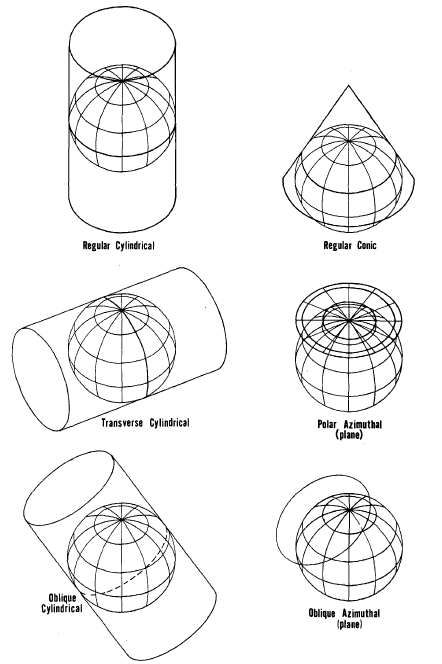
\includegraphics[width=0.8\textwidth,keepaspectratio]{images/methods/mappings.png}
\caption[
    Projection of the earth onto the three major surfaces \iacite{Snyder1987}.
]{Projection of the earth onto the three major surfaces.}
\label{fig:projections-base}
\end{figure}

\subsubsubsection{Cylindrical map projections}
The main concept of cylindrical map projections consist "[\ldots] of meridians which are equidistant parallel straight lines, crossed at right angles by straight parallel lines of latitude, generally not equidistant \iacite{Snyder1987}".
In general, cylindrical map projections can be thought of unrolling a cylinder which has been wrapped around a geoid, touching at the equator (see figure \ref{fig:projections-base} on page \pageref{fig:projections-base}). The following list will feature some projections accordingly to cylindrical projections with a short description taken from \citeauthor{Snyder1987} \iacite{Snyder1987}:

\begin{enumerate}

\ditem{Mercator Projection} \hfill \\
    \begin{itemize}
        \item Cylindrical
        \item Conformal
        \item Meridians are equally spaced straight lines
        \item Parallels are unequally spaced straight lines
        \item Scale is only true along the equator
        \item Loxodromes are straight lines
        \item Not perspective
        \item Poles are at infinity; great distortion of area in polar regions.
    \end{itemize}

    The major advantage according to \citeauthor{Snyder1987} is the navigational feature that loxodromes are straight lines.

\ditem{Transverse Mercator Projection} \hfill \\
    \begin{itemize}
        \item Cylindrical (transverse)
        \item Conformal
        \item Central meridian, each meridian $90^{\circ}$ from central meridian, and equator are straight lines
        \item Other meridians and parallels are complex curves
        \item Scale is true along central meridian
        \item Scale becomes infinite on sphere $90^{\circ}$ from central meridian
    \end{itemize}
\end{enumerate}

\subsubsubsection{Conic map projections}

\subsubsubsection{Azimuthal and related map projections}






